\documentclass{estilo}
\usepackage[spanish]{babel}
\usepackage{graphicx}
\usepackage{float}
\usepackage{amsmath}        % para los vectores columnas
\usepackage{amsfonts}       % para las negrita de pizarra
\usepackage{amssymb}        % para simbolos matematicos
\usepackage{hyperref}       % para utilizar referencias
\usepackage{multirow}       % para las tablas
\usepackage{dsfont}
\usepackage{listings}
\usepackage{xcolor}
\definecolor{codegreen}{rgb}{0,0.6,0}
\definecolor{codegray}{rgb}{0.5,0.5,0.5}
\definecolor{codepurple}{rgb}{0.58,0,0.82}
\definecolor{backcolour}{rgb}{0.95,0.95,0.92}
\lstdefinestyle{mystyle}{
    backgroundcolor=\color{backcolour},   
    commentstyle=\color{codegreen},
    keywordstyle=\color{magenta},
    numberstyle=\tiny\color{codegray},
    stringstyle=\color{codepurple},
    basicstyle=\ttfamily\footnotesize,
    breakatwhitespace=false,         
    breaklines=true,                 
    captionpos=b,                    
    keepspaces=true,                 
    numbers=left,                    
    numbersep=5pt,                  
    showspaces=false,                
    showstringspaces=false,
    showtabs=false,                  
    tabsize=2
}
\lstset{style=mystyle}

\usepackage{enumitem,multicol,setspace}
\newcounter{subenum}[enumi] % para las multicolumnas
\renewcommand{\thesubenum}{\arabic{subenum}}
\usepackage[nomessages]{fp}
\FPeval\thecolwidth{round(1/4:4)}% Specify number of columns -> column width
\newcommand{\newitem}[1]{%
  \refstepcounter{subenum}%
  \parbox{\dimexpr\thecolwidth\linewidth-.5\columnsep}{%
    \makebox[\labelwidth][r]{(\thesubenum)\hspace*{\labelsep}}%
    #1}\hfill%
}

\usepackage{scalerel,stackengine} % para el sombrero
\stackMath
\newcommand\rhat[1]{%
\savestack{\tmpbox}{\stretchto{%
  \scaleto{%
    \scalerel*[\widthof{\ensuremath{#1}}]{\kern-.6pt\bigwedge\kern-.6pt}%
    {\rule[-\textheight/2]{1ex}{\textheight}}%WIDTH-LIMITED BIG WEDGE
  }{\textheight}% 
}{0.5ex}}%
\stackon[1pt]{#1}{\tmpbox}%
}
\parskip 1ex

\usepackage{mathtools}      % floor y ceil
\DeclarePairedDelimiter\ceil{\lceil}{\rceil}
\DeclarePairedDelimiter\floor{\lfloor}{\rfloor} 

\usepackage[style=authoryear-comp]{biblatex}


\begin{document}
\maketitle

\justifying{}

%Tabla de contenidos
\newpage
\tableofcontents % Índice general
\newpage

\newpage
\section*{Consigna}


{\huge Introducción y primeros años}
\vskip0.5cm

Cuando Mateo nació, Sophia estaba muy contenta. Finalmente tendría un hermano con quien jugar. Sophi tenía 3 años cuando Mateo nació. Ya desde muy chicos, ella jugaba mucho con su hermano.

Pasaron los años, y fueron cambiando los juegos. Cuando Mateo cumplió 4 años, el padre de ambos le explicó un juego a Sophia: Se dispone una fila de $n$ monedas, de diferentes valores. En cada turno, un jugador debe elegir alguna moneda. Pero no puede elegir cualquiera: sólo puede elegir o bien la primera de la fila, o bien la última. Al elegirla, la remueve de la fila, y le toca luego al otro jugador, quien debe elegir otra moneda siguiendo la misma regla. Siguen agarrando monedas hasta que no quede ninguna. Quien gane será quien tenga el mayor valor acumulado (por sumatoria).

El problema es que Mateo es aún pequeño para entender cómo funciona esto, por lo que Sophia debe elegir las monedas por él. Digamos, Mateo está “jugando”. Aquí surge otro problema: Sophia es muy competitiva. Será buena hermana, pero no se va a dejar ganar (consideremos que tiene 7 nada más). Todo lo contrario. En la primaria aprendió algunas cosas sobre algoritmos greedy, y lo va a aplicar.
\vskip0.5cm
{\huge Consigna}
\vskip0.5cm
1. Hacer un análisis del problema, y proponer un algoritmo greedy que obtenga la solución óptima al problema planteado: Dados los 
$n$ valores de todas las monedas, indicar qué monedas debe ir eligiendo Sophia para si misma y para Mateo, de tal forma que se asegure de ganar siempre. Considerar que Sophia siempre comienza (para sí misma).
\vskip0.3cm
2. Demostrar que el algoritmo planteado obtiene siempre la solución óptima (desestimando el caso de una cantidad par de monedas de mismo valor, en cuyo caso siempre sería empate más allá de la estrategia de Sophia).
\vskip0.3cm
3. Escribir el algoritmo planteado. Describir y justificar la complejidad de dicho algoritmo. Analizar si (y cómo) afecta la variabilidad de los valores de las diferentes monedas a los tiempos del algoritmo planteado.
\vskip0.3cm
4. Analizar si (y cómo) afecta la variabilidad de los valores de las diferentes monedas a la optimalidad del algoritmo planteado.
\vskip0.3cm
5. Realizar ejemplos de ejecución para encontrar soluciones y corroborar lo encontrado. Adicionalmente, el curso proveerá con algunos casos particulares que deben cumplirse su optimalidad también.
\vskip0.3cm
6. Hacer mediciones de tiempos para corroborar la complejidad teórica indicada. Agregar los casos de prueba necesarios para dicha corroboración. Esta corroboración empírica debe realizarse confeccionando gráficos correspondientes, y utilizando la técnica de cuadrados mínimos. Para esto, proveemos una explicación detallada, en conjunto de ejemplos.
\vskip0.3cm
7. Agregar cualquier conclusión que les parezca relevante.


\newpage

\justifying{
\hypertarget{res}{\section*{Resolución}}
\section{Algoritmo greedy para la resolución del problema}

El problema que se nos presenta en resumidas cuentas es el siguiente:

En un juego por turnos, se nos da una fila con monedas y solo puedo sacar una de uno de los extremos de la fila por turno. El juego termina cuando no quedan más monedas, y gana el jugador que haya acumulado la mayor ganancia.

Recordemos que un algoritmo greedy, es aquel que al aplicar una regla sencilla, nos permita obtener el óptimo local a mi estado actual, y aplicando iterativamente esa regla, llegar a (idealmente) un óptimo global.

Entonces, un algoritmo greedy para resolver el problema, podría ser el siguiente: Vemos las monedas de ambos extremos (mi información actual), y me quedo con la de mayor valor cuando es el turno de Sophia, y la de menor valor cuando es el turno de Mateo (está seria nuestra regla sencilla), la cual aplicamos reiterativamente (hasta que no haya monedas) para llegar a una solución óptima (que Sophia gane siempre).

\section{Demostración del Algortimo}

El algortimo desarrollado anteriormente nos afirma que nos va a dar la solución óptima,
osea que Sophia gana todas las partidas de su nuevo juego, no importa el orden de los valores
de las monedas, dejando a Mateo como el perdedor tanto de cada ronda como del juego en si.

\vskip0.5cm

A continuación, se detallará el paso a paso de la demostración que hemos realizado para afirmar la teoría:

\vskip0.5cm

{\large{Sophia siempre gana las partidas, por lo tanto también el juego}}.
\vskip0.5cm
Utilizamos el método por inducción:
\vskip0.5cm

Siendo $n$ la cantidad de monedas:
\vskip0.5cm

Si $n=1$ 


\includegraphics[width=6.5cm, height=4cm]{images/IMG_1625.jpg}


$valorSophiaMonedas=M_{1}$

$valorMateoMonedas=0$

Gana Sophia ya que siempre el primer turno es para ella, y solo hay una moneda.

\vskip1cm

Si $n=2$


\includegraphics[width=6cm, height=3cm]{images/IMG_1626.jpg}

Siendo, $M_{1}>M_{2}$ : 


$valorSophiaMonedas=M_{1}$

$valorMateoMonedas=M_{2}$

Al empezar Sophia, ella agarra la moneda más grande y gana
\vskip1cm
Si $n=3$


\includegraphics[width=6.5cm, height=3cm]{images/IMG_1627.jpg}

Siendo, $M_{1}<M_{2}<M_{3}$ : 


$valorSophiaMonedas=M_{3}+M_{2}$

$valorMateoMonedas=M_{1}$

Sophia agarra $M_{3}$ al ser el más grande, Mateo agarra (en realidad lo elige Sophia) el $M_{1}$ que es el valor
más pequeño, y por último Sophia agarra la moneda $M_{2}$ que es la última que quedaba. 
Sophia gana al tener las monedas de mayor valor.

\vskip1cm
Si $n=4$

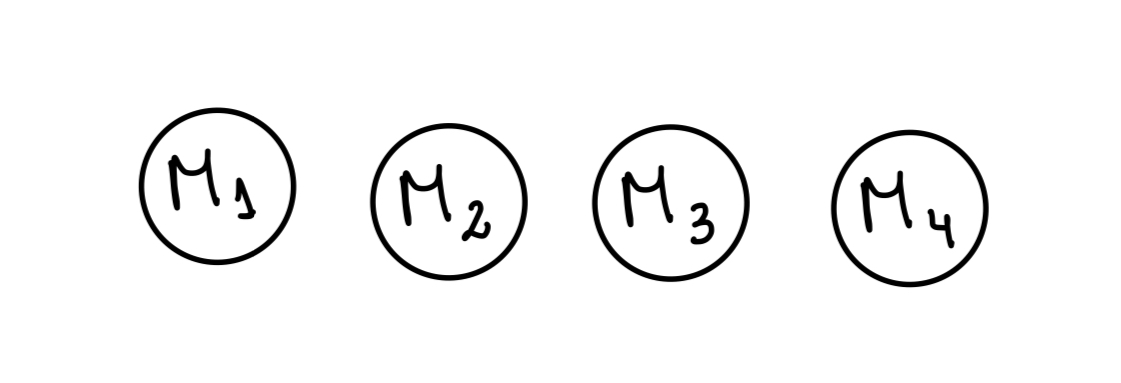
\includegraphics[width=8.5cm, height=3.5cm]{images/IMG_1628.jpg}

Siendo, $M_{4}<M_{3}<M_{1}<M_{2}$ : 

$valorSophiaMonedas=M_{1}+M_{2}$

$valorMateoMonedas=M_{4}+M_{3}$

Sophia agarra $M_{1}$ al ser la mas grande en comparación a $M_{4}$; Mateo agarra la moneda $M_{4}$ al ser la mas 
pequeña entre $M_{4}$ y $M_{2}$; Sophia agarra $M_{2}$ y por último (por descarte) Mateo se queda con la moneda $M_{3}$.
Gana Sophia por tener el mayor valor de monedas.

\vskip1cm
Si $n=k$

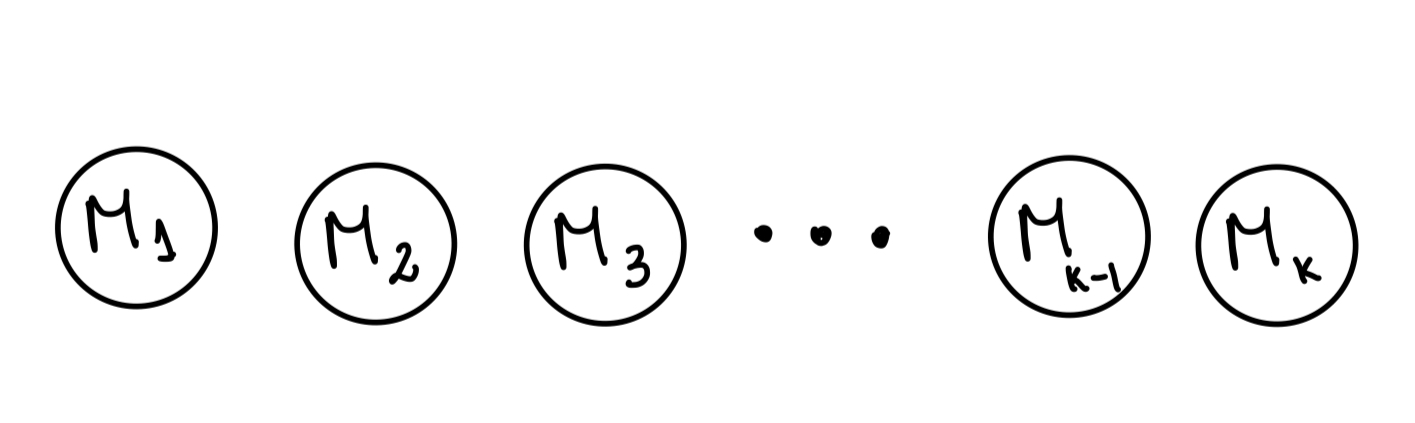
\includegraphics[width=9cm, height=3.5cm]{images/IMG_1629.jpg}

No podemos establecer quien es mayor/menor al haber k valores, ya que en la fila los valores no están ordenados de forma ascendente o descendentemente.

Para poder analizarlo vamos a hacer una función partida para ver cuales son nuestras opciones para cada uno:

$ValorSophiaTurno= \left\{ \begin{array}{lcc} M_{k} & si & M_{k}>M_{1} , ValorMateoTurno= \left\{ \begin{array}{lcc} M_{k-1} & si & M_{k-1}<M_{1} \\ \\ M_{1} & si & M_{k-1} > M_{1} \end{array} \right. \\ \\ M_{1} & si & M_{k} < M_{1}, ValorMateoTurno= \left\{ \begin{array}{lcc} M_{2} & si & M_{2}<M_{k} \\ \\ M_{k} & si & M_{k} < M_{2} \end{array} \right. \end{array} \right.$
\vskip0.3cm
En consecuencia del turno de Sofía, Mateo va a tener 2 posibilidades por cada elección.
\vskip0.7cm
Como podemos observar, siempre hay un patrón: Si los turnos empezaran desde el 0, Sophia siempre tiene los turnos pares, en los cuales agarra las monedas de mayor valor, y Mateo tiene los turno impares donde agarra las monedas de menor valor.

\vskip0.5cm

\vskip0.5cm
$valorSophiaTotal =  \sum_{k=1}^{n}M_{k}$ siendo $\left\{ \begin{array}{lcc} k=i_{inicial\_actual} & si & i_{inicial\_actual}>j_{final\_actual} \\ \\ k=j_{final\_actual} & si & i_{inicial\_actual}<j_{final\_actual} \end{array} \right.$

\vskip0.5cm
$valorMateoTotal =  \sum_{k=1}^{n}M_{k}$ siendo $\left\{ \begin{array}{lcc} k=i_{inicial\_actual} & si & i_{inicial\_actual}<j_{final\_actual} \\ \\ k=j_{final\_actual} & si & i_{inicial\_actual}>j_{final\_actual} \end{array} \right.$

\vskip0.5cm
\textbf{Nota}: $i_{inicial\_actual}$ es el principio de nuestra fila de monedas por turnos, y $j_{final\_actual}$ en el final de nuestra fila por turnos 
\vskip0.8cm
Y para corroborar que nadie está haciendo trampa, se debe cumplir que:
\vskip0.5cm
\begin{center}
    $valorTotalDeMonedas=valorSophiaTotal+valorMateoTotal$
\end{center}



\section{Algoritmo planteado y complejidad}

El algoritmo que decidimos utilizar para resolver el problema, es el siguiente:

\begin{verbatim}
    def juego_monedas(monedas):
    turno = 0 # Los turnos pares son de Sophia, los impares de Mateo
    i = 0
    j = len(monedas) - 1

    acum_sophia = 0
    acum_mateo = 0
    movimientos = []
    while not (i > j):
        primera_moneda = monedas[i]
        ultima_moneda = monedas[j]
        if turno % 2 == 0:
            if primera_moneda > ultima_moneda:
                acum_sophia += primera_moneda
                i += 1
                movimientos.append("Primera moneda para Sophia")
            else:
                acum_sophia += ultima_moneda
                j -= 1
                movimientos.append("Última moneda para Sophia")
        else:
            if primera_moneda < ultima_moneda:
                acum_mateo += primera_moneda
                i += 1
                movimientos.append("Primera moneda para Mateo")
            else:
                acum_mateo += ultima_moneda
                j -= 1
                movimientos.append("Última moneda para Mateo")
        turno += 1

    return movimientos, acum_sophia, acum_mateo
\end{verbatim}

\begin {itemize}
\item Mientras hayan monedas para elegir:
    \begin {itemize}
    \item Vemos las monedas que se encuentran en los dos extremos de la fila, y las comparamos:
        \begin {itemize}
        \item Si el turno es de Sophia, se elige la moneda de mayor valor.
        \item Si el turno es de Mateo, se elige la moneda de menor valor.
        \end {itemize}
    \end {itemize}
\item Devolvemos la ganancia acumulada de Sophia y Mateo.
\end {itemize}

Lo que estamos haciendo, es recorrer toda la fila de monedas (con dos índices, uno para cada extremo), y en cada iteración, comparamos las monedas, y acumulamos la ganancia para Sophia o Mateo (según corresponda el turno), y se agrega el movimiento que se realizó, hasta que finalmente ya no quedan monedas. Por lo tanto, siendo $n$ las monedas de la fila, nuestro algoritmo es lineal: O(n), ya que solamente recorremos ese arreglo de monedas, y en cada iteración hacemos operaciones de tiempo constante: O(1).

En conclusión, la complejidad algorítmica es: \textbf{O(n)}.
\section{Variabilidad}
\section{Ejemplos de ejecución}

Se pueden encontrar múltiples ejemplos de ejecución dentro de la carpeta \textit{ejemplos} en el repositorio. Veamos alguno:

Supongamos que tenemos 6 monedas:

\begin{lstlisting}
    [3, 7, 1, 12, 9, 5]
\end{lstlisting}

Recordando lo que vimos en la sección 3 de Algoritmo planteado y complejidad, y que el primer turno es de Sophia:

Vemos las monedas de ambos extremos: 3 y 5. Como el turno es de Sophia, nos quedamos con la moneda de mayor valor, en este caso 5. Entonces:  \textbf{Ganancia de Sophia = 5}

Nuestras monedas quedarían ahora:

\begin{lstlisting}
    [3, 7, 1, 12, 9]
\end{lstlisting}

Ahora las monedas de ambos extremos son: 3 y 9. Como ahora es el turno de Mateo, nos quedamos con la moneda de menor valor: 3. Entonces:  \textbf{Ganancia de Mateo = 3}

Nuestras monedas quedarian ahora:

\begin{lstlisting}
    [7, 1, 12, 9]
\end{lstlisting}

Siguiendo el algoritmo hasta el final (hasta que ya no queden monedas), obtenemos finalmente:

\textbf{Ganancia de Sophia = 26} (5 + 9 + 12)

\textbf{Ganancia de Mateo = 11} (3 + 7 + 1)

Como la ganancia de Sophia es mayor que la de Mateo (26 $>$ 11), Sophia resulta la ganadora del juego.

Veamos lo que obtenemos al ejecutar el codigo:

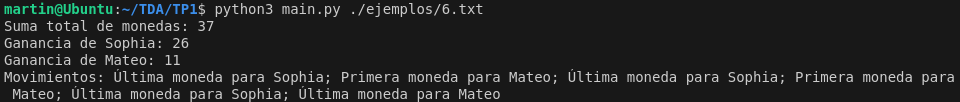
\includegraphics[scale = 0.45]{ {./images/ejemplo_ejecucion_6_monedas} }
\section{Medición empírica}

Para comprobar empíricamente la complejidad \textbf{O(n)} del algoritmo, se decidió ejecutar el mismo con distintos tamaños de entrada y medir el tiempo de ejecución. Se generaron muestras de tamaño n, las cuales varían desde 1 hasta 100 millones.

Para cada muestra se registró el tiempo de ejecución, obteniendo el siguiente gráfico:

\begin{center}
    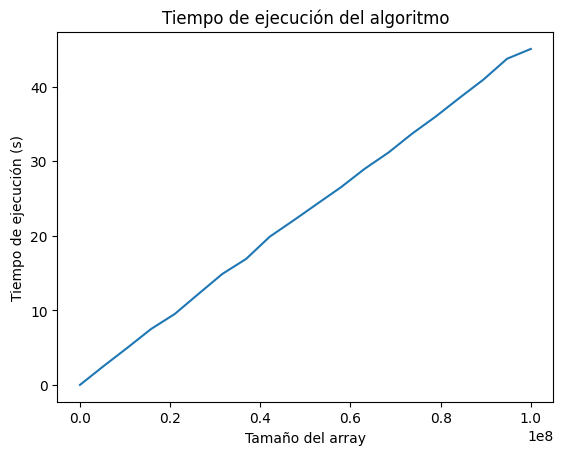
\includegraphics[scale = 0.6]{ {images/tiempoDeEjec.png} }
\end{center}

A simple vista se puede observar un crecimiento lineal. Para confirmar esto, vamos a ajustar los datos a una recta mediante cuadrados mínimos. Esto lo realizamos con Python y la función \textit{optimize.curve\_fit} de la librería \textit{scipy}.

Obtenemos que el gráfico se puede ajustar a la recta $y = 4.54x + 0.25$, con un error cuadrático medio de 0.06. Por lo tanto, podemos concluir que el algoritmo tiene una complejidad \textbf{O(n)}.

\begin{center}
    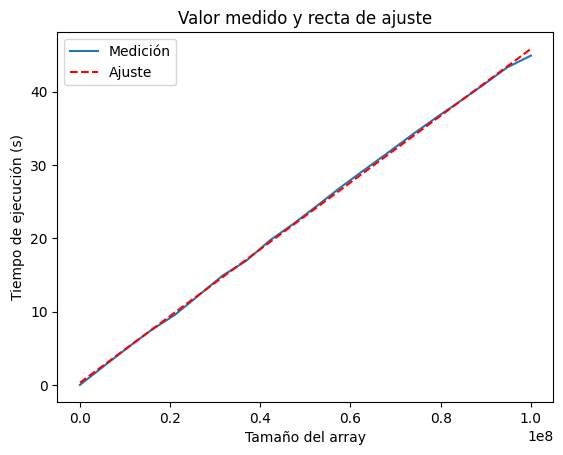
\includegraphics[scale = 0.6]{ {images/cuadradosMinimos.png} } 
\end{center}
\section{Conclusiones}

Acá irían las conclusiones de todo nuestro trabajo :)

}


\newpage
\end{document}